\section{Motivation}
\label{sec:motivation}

Buildings are notoriously complex from a management perspective.  They consume a large fraction
of the energy produced in the United States and much of is wasted~\cite{next10_waste}.  
There has been
much work in the building science community to reduce their energy consumption and make them more
efficient, but the route to broader impact is typically carried out through regulations guided
by the findings of studies in those communities.%~\cite{regulation}.
We aim to let solutions reach buildings \emph{directly} by making sense of the data they produce
as quickly and accurately as possible.
In order to achieve this at scale, we must explore ways to deal with the data produced
from sensors within them and to enable broad analysis across several buildings at a time. Our study
focuses on any building equipped with a network of sensors.  Nearly 
three-quarters of commercial buildings contain a rich sensing fabric, installed as part
of the building management system~\cite{epa}.  
It is the data from these system and variants of it, that
we wish to unify and make sense of in a more systematic and automated fashion.

% walk through an example of point names from 2 or three buildings and explain 
% what's challenging here
%
% BLDA1R435__ART
% BLDA1R435__ARS
% BLDA1R545__ART
%Buildings consume a large fraction of the energy produced in the United States, and much of it
%is wasted\cite{epa}.  
The data problems parallel the complexity of buildings. Ad-hoc data management practices
make it difficult for any analytical solution to be widely ported or run across building
systems.  
%For example, consider the following stream names: \texttt{BLDA1R435\_\_ART,
%BLDA1R435\_\_ARS}. Each name encodes contextual information in the form
%of concatinated character sequences. In these, the first 4 characters refer to the 
%name of the building, the next one encodes the air handling unit association, the next 
%four encode the room,
%and the last three encode the acronym for the type.  Although the examples given are well
%structured, many variants within the same data set exist.  For example, \texttt{BLD\_1R435\_ARG\_}
%is the encoding for a different sensor in the same room as the others, but with a name
%that is \emph{like} although not exactly the same structure as the others.
% Discuss how active learning technique can be used to "unify" these tag names
When dealing with a small number of points such differences are usually not a problem.  Upon 
visual inspection, 
encodings are similar enough that the engineer can decode the meaning.  However, for automatic 
processing or processing a large number of points across buildings, these kinds of 
variations makes it difficult to generalize the character-construction rule set.  
\emph{Fundamentally, full coverage is attainable if we could learn all the codes and map
them to more descriptive search terms.}
%Since many of the codes change from across vendors and buildings, Analytical applications 
%need to make building-specific adjustments in order to run the same analysis job across each
%building.  For example, if we are trying to determine the fraction of uncomfortable rooms
%in each building on our campus, the two collections of sense points we need are the temperature
%sensors and the corresponding set points in each building.  Because the code for temperature
%sensor and the code for set point is slightly different in each building, the query
%must be adjusted each time the job is set to run on the data from a new building.

At a high level we want to normalize the metadata across all buildings so that one query
can run across all of buildings, and we want the normalization process to be automatic, so that
the overhead in adding a new building to the set is small -- the latter of which is important
for achieving scale.  Fundamentally, a tradeoff exists between the degree to which we can 
automate the normalization task and the level of coverage you get in the general 
rule construction.  You can get full coverage with no automation.  This is essentially the approach
that is common today.  Every solution that incorporates a building's data is manually
adjusted, specifically for that particular building.  You can get some degree of coverage if you
use a general set of rules, increasing the automation factor and decrease the manual one.
Tuning is quite arduous and in most cases, non-programmers are tuning the data ingestion script.

The problem for a large number of buildings is particularly pernicious to the goal. Although 
there are some similarities for certain kinds of sensor
labels and metadata, searching across them yields results of varying success.  Consider the 
simplest kind of a search, a grep scan across the metadata associated with the points
across a set of buildings.  If we wish to attain all the temperature sensors or set points
for a particular building, without knowing these codes, we should be able to attain
it by search for all points in a particular building that measure ''temperature`` or
that have ``setpoint'' in their description.

We demonstrate this by collecting all the metadata across our building
testbed.  The testbed consists of almost 60 buildings and over 20,000 sense points.  We collected
the names for each of the set points and any associated metadata that describes the meaning
of the name.  Then, we run a number of grep searches on the data and calculate the 
relative success of the query.  Figure~\ref{fig:sodagrep} shows the results for two queries.
The `temperature` grep string is ``buildingA room temp'' and the `setpoint` grep string
is ``buildingA room setpoint''.  For the temperature query we attain 87.5\% of the 
actual sense points we are searching for, while for the setpoint query we attain only 56\%
of the setpoints in the building.  We could try different search queries that yield different
results, however, because there's only \emph{some} overlapping metadata terms across
buildings, coverage tends to be quite poor.

\begin{figure}[h!]
\centering
    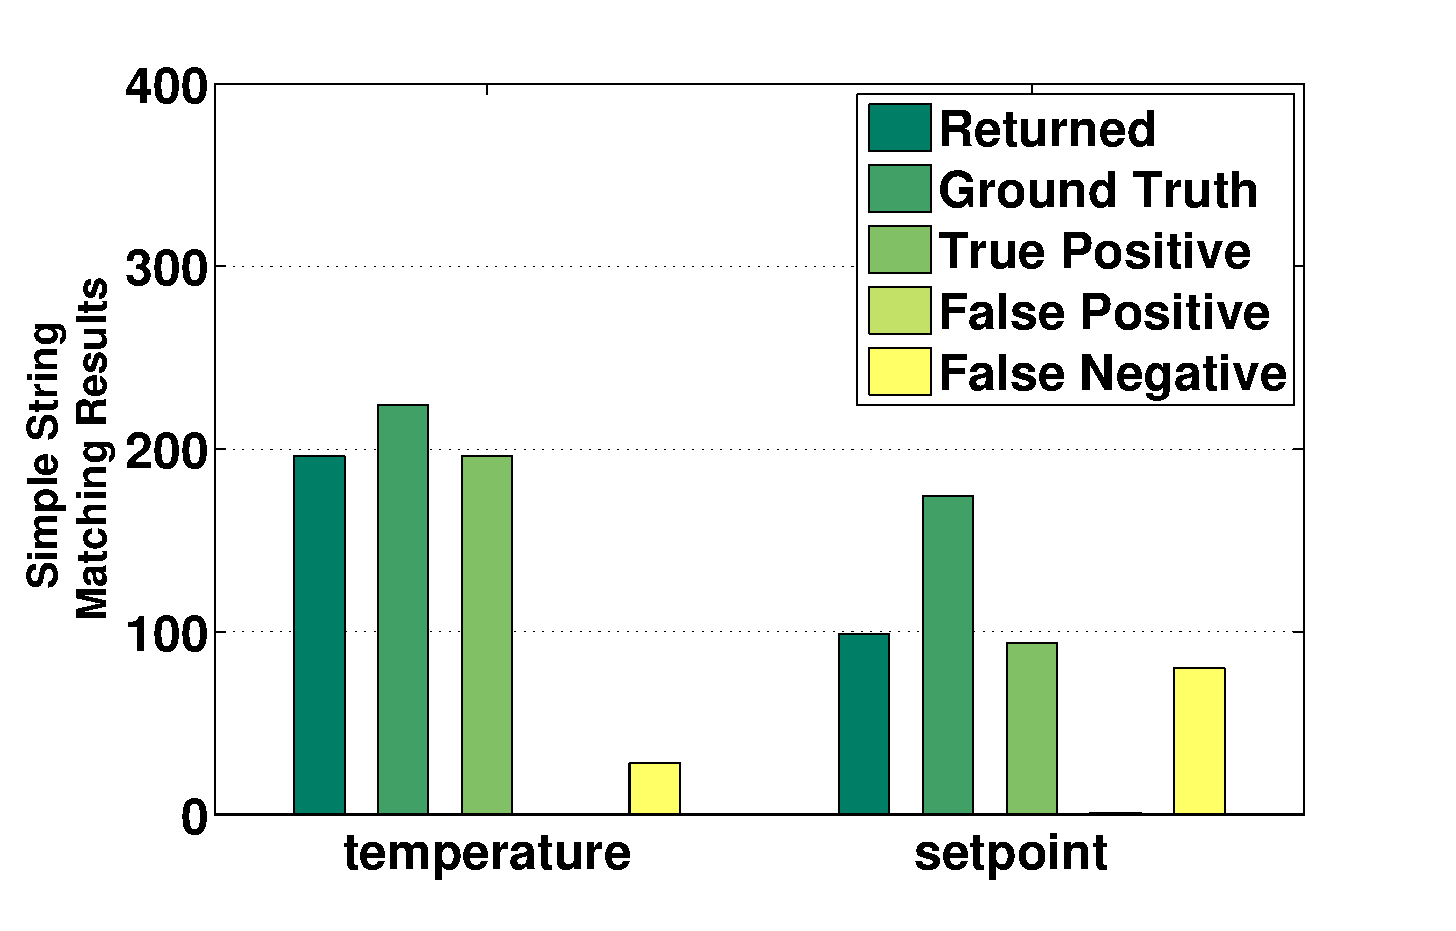
\includegraphics[width=0.48\textwidth]{figs/soda_grep_result.eps}
    \caption{Results when running a grep search on the point names in a single building.}
\label{fig:sodagrep}
\end{figure}

% write a couple of paragraphs about why programming by example and 
% input-output stuff here
A key observation we have made while attempting to write ingestion scripts in that 
we create a program $P_{1}$ to that parses the data and generates a set of point names
$n_{1}$ with coverage $c_{1}$ of the points we need to obtain.  We notice there are
points missing, so we write another program $P_{2}$ that generates another set of points
$n_{2}$ which includes some of all of the points in $n_{1}$ and gives us coverage $c_{2}$.
We keep noticing there are points missing and keep either expanding or adjusting
the program to get closer and closer to full coverage.  In practice, the coverage is not
easily attainable without an expert, familiar with the data set, inspecting the results.
So the challenge is to attain the good coverage in one (or a few) buildings using input-out
examples, using a technique similar
to the work by Gulwani et al~\cite{Gulwani:2011}, and use this the resulting program and
a few more example in each building to have the process learn the variants of all the codes
and boost them with extra tags that are learned from other buildings.

This process allows us to leverage the knowledge of the expert while minimizing the integration
overhead per building.  Moreover, as more examples the provided, the better that 
algorithm can learn how to cover a broader set of codes and boost them with common tags.
Also, the technique used in previous work is well suited for our problem, since
users tend to be non-programmers.  The input-output example interactive model is well suited
for interacting with non-programmers and getting the kind of information we need from them
to automate the program creation process to learn the various point code. 

%Without rule-set construction the data cannot be ingested properly or interpretted
%correctly.  
%However, there are ``active learning'' techniques in the literature~\cite{ms} 
%that address this problem by leveraging the knowledge of an expert. The idea behind active learning
%is that you can request input from an expert to improve the accuracy of your algorithm.
%In the case of name/tag expansion you 
%can generalize the set of rules that generate a name/tag by example, iteratively
%updating the name construction rule set for different types of names.  An expert feeds
%the system examples of names for a particular type of sensor or code, and the algorithms 
%that generalize the character-set construction rules can raise the confidence of the
%expanded expression.
%We explore the use
%of \emph{active learning} techniques to iteratively learn all the variants within an across
%data sets.

%Fortunately, we have access to a large corpus of data from buildings on our campus.

\section{Building Testbed}
In our experiments we used an extensive building testbed that 
consists of 56 buildings containing over 16,000 sense points. These buildings 
represent a vast range in age, size, and density of deployment.  It also represents deployments
that were set up by more than one vendor.  As expected, newer buildings have many more sense 
points than older ones -- although some old buildings that have been retrofitted have over 1000  
points within them. The general trend in the number of sense points versus the year the 
building is built is roughly linearly increasing in the log of the number of points, as shown
in Figure~\ref{fig:sense_pts_data_yb}.  

\begin{figure}[htb!]
\centering
	\begin{subfigure}{0.48\textwidth}
                \centering
		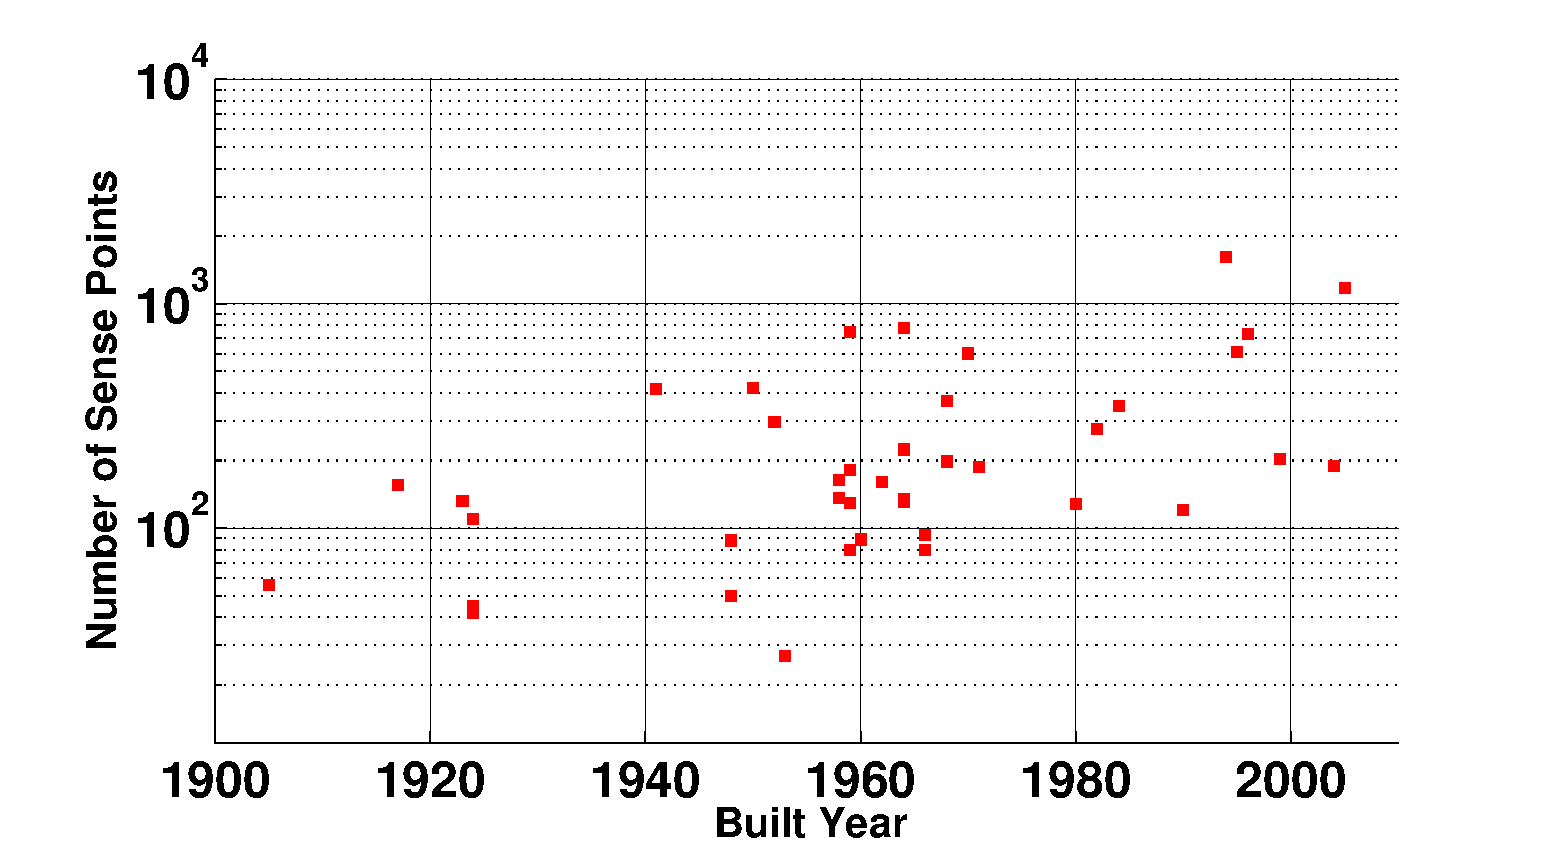
\includegraphics[width=\textwidth]{./figs/pts_vs_yearbuilt.eps}
                \caption{Number of Points vs Year Built}
                \label{fig:sense_pts_data_yb}
	\end{subfigure}
	\begin{subfigure}{0.48\textwidth}
                \centering
		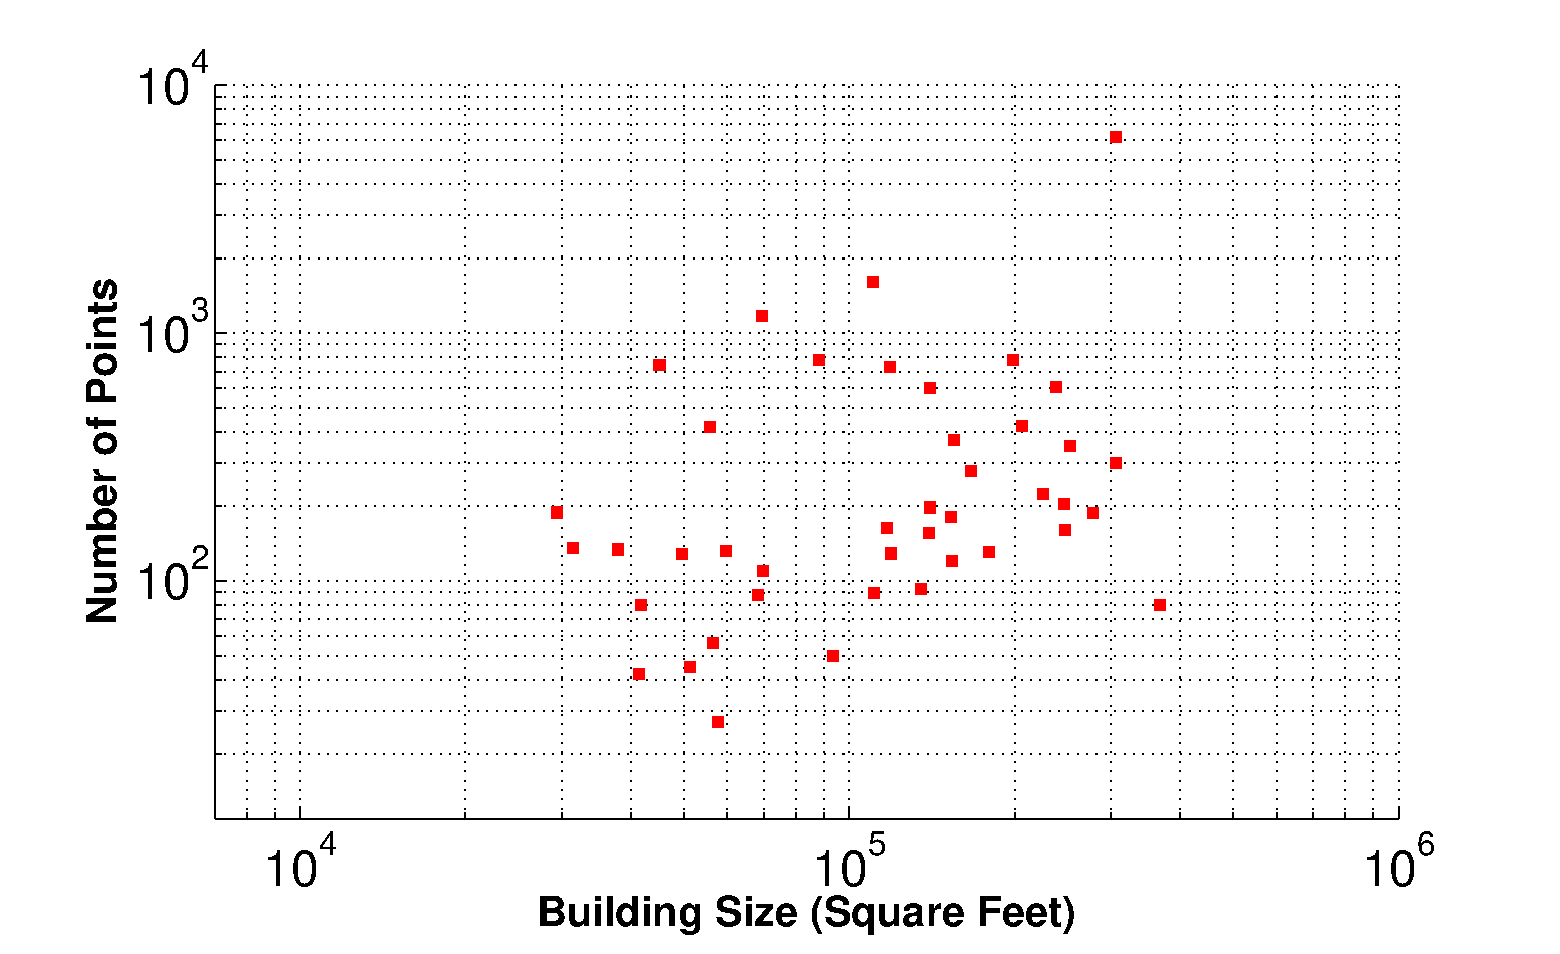
\includegraphics[width=\textwidth]{./figs/pts_vs_buildsz.eps}
                \caption{Number of Points vs Building Size}
                \label{fig:sense_pts_data_bs}
	\end{subfigure}
\caption{Relationship between the built year and the building size on the number of sense
points.  This data is summarize from a testbed that we used for experiments that consists of
almost 60 buildings and over 16,000 sense points.}
\label{fig:sense_pts_data}
\end{figure}

The maximum number of points in a 
single building is 1614 and the minimum is 27.   The built years spans over 100 years -- from 
1905 to 2005. The size range spans over an order of magnitude 
in square footage from about 30,000 square feet to over 360,000 square feet.  There is no
observable correlation between the size of the building and the number of sense points.
Figure~\ref{fig:sense_pts_data_bs} shows a log-log plot of the number of points versus
the size of the building.  There is one large building with many sense points, but the size
seems to have little to do with the density of the deployment.
The access this
this kind of breadth of system and building types makes our study unique.


% expand the discussion to include sensor sin iot?


% Now discuss how the actual shapes of the readings can be quite similar looking



%\begin{figure}[h!]
%\centering
%    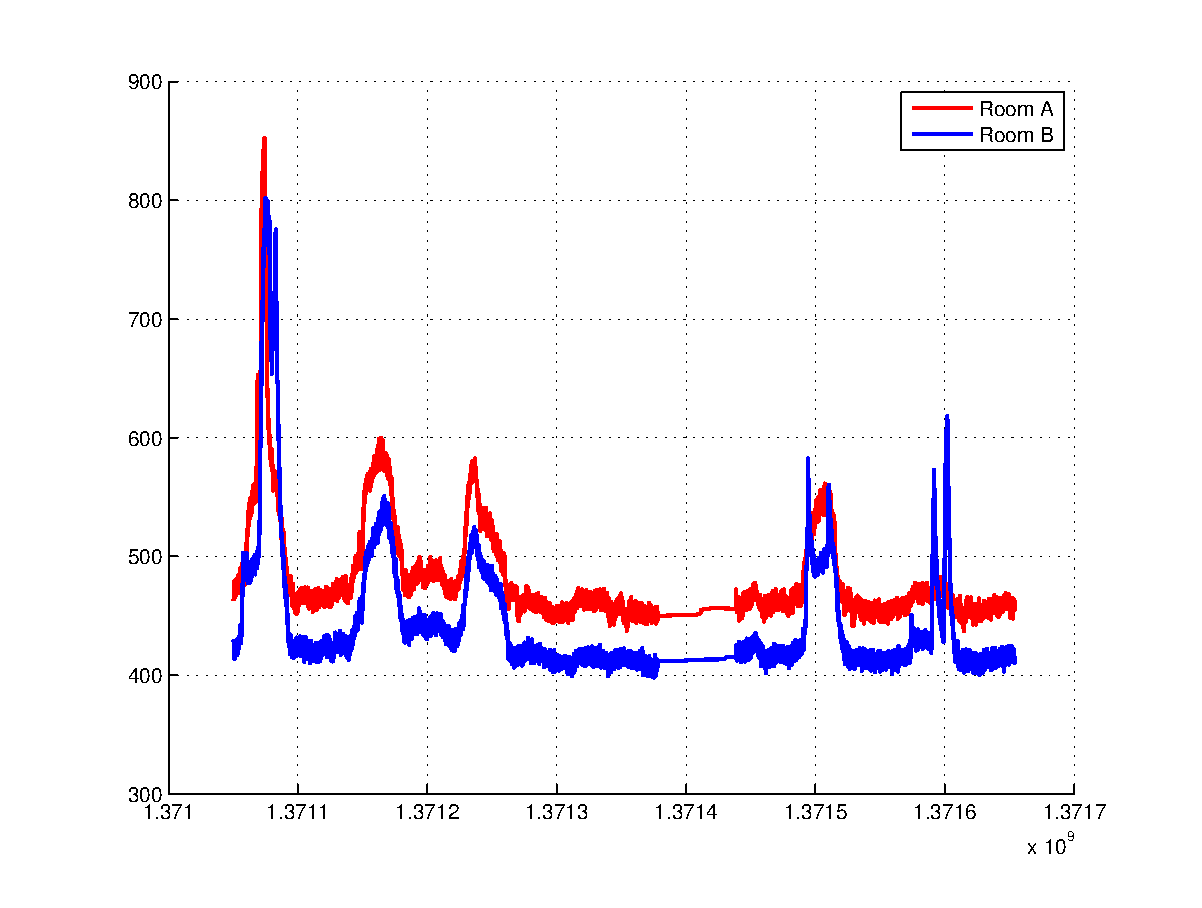
\includegraphics[width=0.48\textwidth]{figs/co2_pair.eps}
%    \caption{CO2 sensor traces.}
%\label{fig:co2traces}
%\end{figure}
%
%\begin{figure}[h!]
%\centering
%    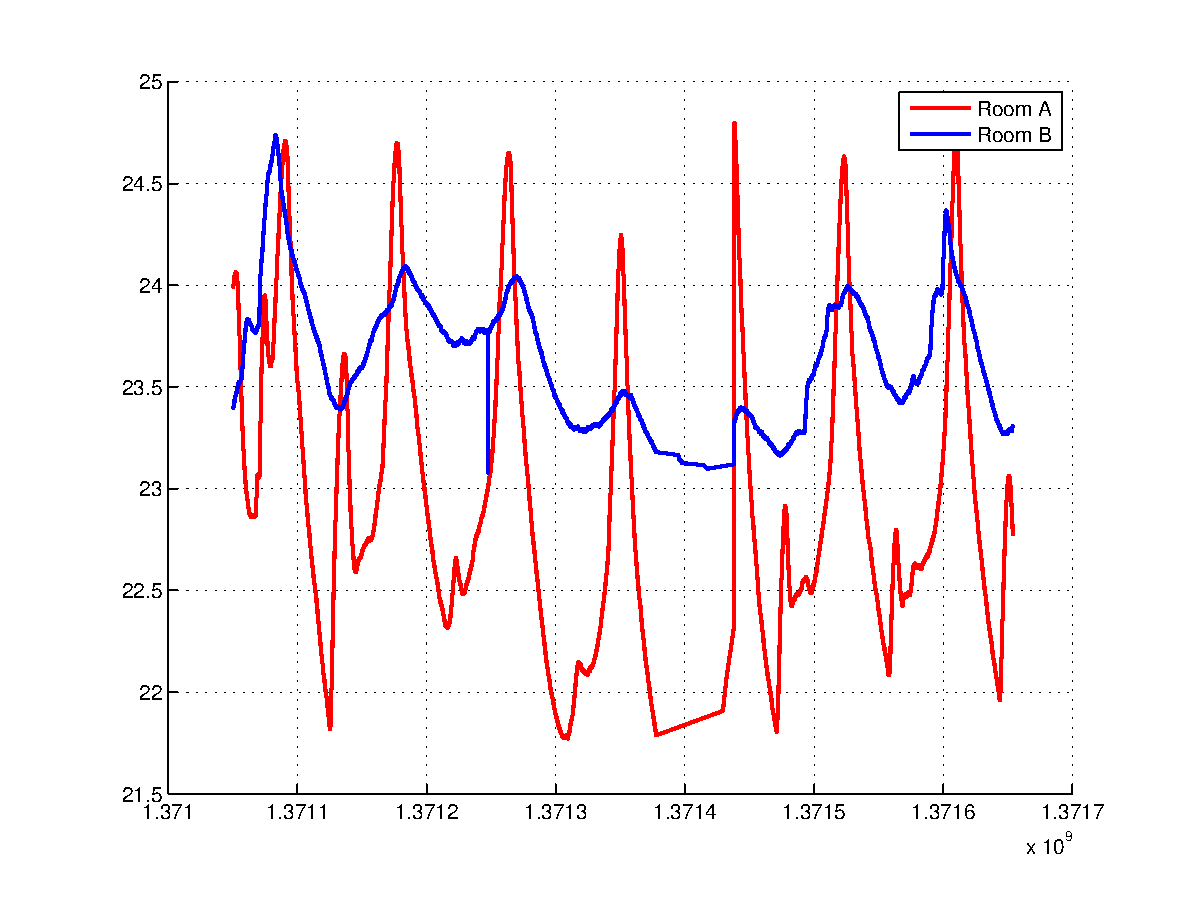
\includegraphics[width=0.48\textwidth]{figs/temp_pair.eps}
%    \caption{temperature traces.}
%\label{fig:temptraces}
%\end{figure}

% tie this into search; search is done for scale
% scale is necessary for broad impact
% 

% discuss how both can be used to generate more metadata that we can use for indexing


